\documentclass[border={0.1cm 0.1cm 0.1cm 0.1cm}]{standalone}  %E,S,W,N

\usepackage{amssymb}
\usepackage{amsmath}
\usepackage{tikz}
\usepackage{xcolor}
\definecolor{rosewood}{rgb}{0.4,0.0,0.04}

\begin{document}
	
	%BEFORE LIGHTING
	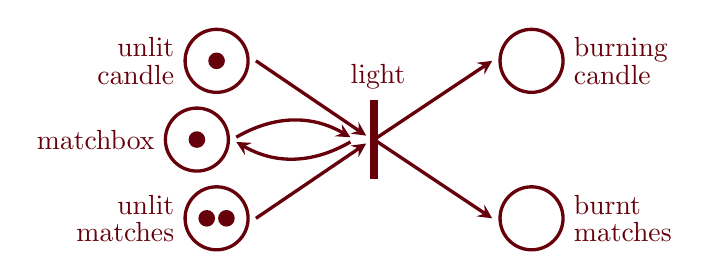
\begin{tikzpicture}[rosewood,very thick]	
	%STATES
	\draw (-2, 1) circle (0.4cm) node[left,align=right,xshift=-.4cm] {unlit \\[-0.75mm] candle};
	\draw (-2.25,0) circle (0.4cm) node[left,align=right,xshift=-.4cm] {matchbox};
	\draw (-2,-1) circle (0.4cm) node[left,align=right,xshift=-.4cm] {unlit \\[-0.75mm] matches};
	\draw ( 2, 1) circle (0.4cm) node[right,align=left,xshift=0.4cm] {burning \\[-0.75mm] candle};
	\draw ( 2,-1) circle (0.4cm) node[right,align=left,xshift=0.4cm] {burnt \\[-0.75mm] matches};
	
	%LEFT ARCS
	\draw[->,>=stealth] (-1.5, 1)--(-0.1,0.05);
	\draw[->,>=stealth] (-1.5,-1)--(-0.1,-.05);
	%
	\draw[->,>=stealth] (-1.75,0.03) to[bend left ] (-0.3,0.03);
	\draw[<-,>=stealth] (-1.75,-.03) to[bend right] (-0.3,-.03);
	
	%TRANSITION
	\fill (-0.05,-0.5) rectangle (0.05,0.5) node[above] {light}; %transition
	
	%RIGHT ARCS
	\draw[->,>=stealth] (0,0)--(1.5, 1); %light -- candle
	\draw[->,>=stealth] (0,0)--(1.5,-1); %light -- matches
	
	%TOKENS
	\fill (-2,1) circle (3pt); %candle
	\fill (-2.25,0) circle (3pt); %matchbox
	\fill (-2.125,-1) circle (3pt); \fill (-1.875,-1) circle (3pt); %matches
	\end{tikzpicture}%
	%
	\hspace{1cm}%
	%
	%AFTER LIGHTING
	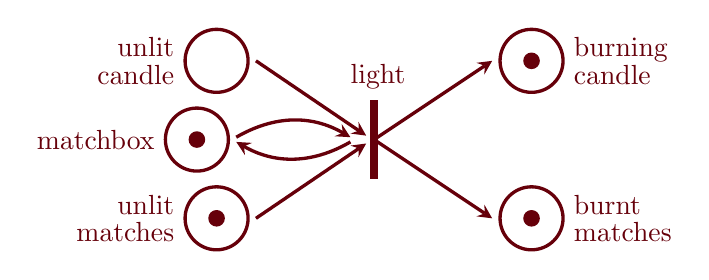
\begin{tikzpicture}[rosewood,very thick]	
	%STATES
	\draw (-2, 1) circle (0.4cm) node[left,align=right,xshift=-.4cm] {unlit \\[-0.75mm] candle};
	\draw (-2.25,0) circle (0.4cm) node[left,align=right,xshift=-.4cm] {matchbox};
	\draw (-2,-1) circle (0.4cm) node[left,align=right,xshift=-.4cm] {unlit \\[-0.75mm] matches};
	\draw ( 2, 1) circle (0.4cm) node[right,align=left,xshift=0.4cm] {burning \\[-0.75mm] candle};
	\draw ( 2,-1) circle (0.4cm) node[right,align=left,xshift=0.4cm] {burnt \\[-0.75mm] matches};
	
	%LEFT ARCS
	\draw[->,>=stealth] (-1.5, 1)--(-0.1,0.05);
	\draw[->,>=stealth] (-1.5,-1)--(-0.1,-.05);
	%
	\draw[->,>=stealth] (-1.75,0.03) to[bend left ] (-0.3,0.03);
	\draw[<-,>=stealth] (-1.75,-.03) to[bend right] (-0.3,-.03);
	
	%TRANSITION
	\fill (-0.05,-0.5) rectangle (0.05,0.5) node[above] {light}; %transition
	
	%RIGHT ARCS
	\draw[->,>=stealth] (0,0)--(1.5, 1); %light -- candle
	\draw[->,>=stealth] (0,0)--(1.5,-1); %light -- matches
	
	%TOKENS
	\fill ( 2, 1) circle (3pt); %candle (burning)
	\fill (-2.25,0) circle (3pt); %matchbox
	\fill (-2,-1) circle (3pt); %matches (unlit)
	\fill ( 2,-1) circle (3pt); %matches (unlit)
	\end{tikzpicture}
	
\end{document}